%!TEX root = "../../DA_GUI.tex"

%	--------------------------------------------------------
% 	Aufbau der Benutzeroberfläche
%	--------------------------------------------------------

\chapter{Elemente der Benutzeroberfläche}
In diesem Kapitel wird der grundlegende Aufbau der Fenster und Benutzeroberflächen von C Compact beschrieben - sowohl die konzeptuelle Konstruktion als auch die Implementierung.
\section{Das Konzept}
Das Aussehen und die Bedienung von C Compact folgt durchgehend der grundlegenden Idee, eine einfach und intuitiv zu bedienende Entwicklungsumgebung zu schaffen. Das bedeutet, Features möglichst zielgruppenorientiert zu integrieren und überflüssige Funktionen zu vermeiden. Bei der Entwicklung wurde besonders auf Vollständigkeit und logische Bedienvorgänge geachtet, um eine konsistente und verständliche Bedienung zu ermöglichen.
% read last sentence
%Durch besondere Rücksicht auf Vollständigkeit und logische Bedienvorgänge haben wir ein durchgängig logisches Bedienerlebnis angestrebt.
%Konkret haben wir uns dabei an folgende Regeln gehalten:

C Compact wurde deshalb nach folgenden Richtlinien entwickelt:
\begin{itemize}
\item Das Aussehen und die Positionierung von Elementen in der Benutzeroberfläche soll logisch begründbar sein
\item Funktionen, die im FSST-Unterricht der ersten und zweiten Klassen wahrscheinlich nicht benötigt werden, werden vermieden oder sind standardmäßig deaktiviert; Bedienelemente werden also auf das Wesentlichste reduziert
\item Wir sind der Meinung, dass eine intuitiv zu bedienende Oberfläche nicht durch Animationen und große Symbole erzielt werden kann, sondern durch einfache, bereits bekannte Konzepte. So sind in C Compact bekannte Elemente wie beispielsweise eine Menüleiste mit gewohnten Datei- und Dokumentoperationen zu finden (Siehe Kapitel \ref{sec:gui-main-menu}).
\end{itemize}

\subsection{Daraus resultierende Einschränkungen}
Durch diese Reduktion der gesamten Oberfläche ist C Compact auf einen bestimmten Zweck, die Ausbildung, beschränkt. Das sehen wir allerdings nicht als Nachteil, sondern als besondere Stärke. Mit C Compact wollen wir eine Entwicklungsumgebung schaffen, die Anfänger nicht überfordert und ihnen hilft, sich auf das Wesentliche zu konzentrieren.
Das Konzept einer anfängerfreundlichen Entwicklungsumgebung ist mit dem Aufbau einer Umgebung für die professionelle Entwicklung nicht vereinbar. C Compact soll aber auf späteres Arbeiten mit komplexeren Programmen vorbereiten. Schüler, die ihre erste Programmiersprache mit C Compact erlernen, kennen bereits den Umgang mit einem Debugger und haben ein tieferes Verständnis für den Ablauf von Programmen.

\section{Fenster Der Benutzeroberfläche}
Neben dem Hauptfenster, das den Kern der Benutzeroberfläche darstellt, gibt es eine Reihe von kleineren Aktionsfenster, Dialogen und Einstellungsfenstern, die zum reibungslosen Ablauf bei der Bedienung von C Compact beitragen. Das Hauptfenster selbst wird in Kapitel \ref{sec:gui-main} beschrieben.

\section{Launcher}
Der Launcher ist ein eigenes Fenster, welches vor dem Öffnen der Benutzeroberfläche angezeigt wird. Hier hat der Benutzer die Möglichkeit, eigene Profile zu erstellen, die Sprache zu ändern und sein Benutzerprofil zu starten. Auch werden hier die zuletzt geöffneten Profile dargestellt.

\begin{figure}[h] 
  \centering
     \includegraphics[width=0.9\textwidth]{./media/images/gui/launcher/launcher_main.png}
  \caption{Launcher GUI}
  \label{fig:launcher_GUI}
\end{figure}

%TODO Verwei auf Anhang
Grundsätzlich ist der Launcher ein JFrame\footnote{\url{http://www.java-tutorial.org/jframe.html}}, das vor dem Start der Benutzeroberfläche angezeigt wird. Die zuletzt verwendeten Profile werden mithilfe einer JScrollpane\footnote{\url{http://www.java2s.com/Tutorial/Java/0240__Swing/CreatingaJTable.htm}}  in welcher mehrere JPanels\footnote{\url{https://docs.oracle.com/javase/tutorial/uiswing/components/panel.html}} liegen, angezeigt. In den JPanels befinden sich der Name und das Benutzerbild.

\begin{itemize}
\item Falls in der Liste, kein Profil vorhanden ist, wird auf die Erstellung eines neuen Profils hingewiesen.
\item Wenn der Benutzer kein Profilbild gewählt hat, wird ein voreingestelltes Profilbild verwendet.
\item Mit einem Klick auf das Profilbild kann das gewünschte Profil geöffnet werden.
\item Es besteht die Möglichkeit, C Compact mithilfe des Launchers ohne Profil zu starten. Das bedeutet, dass kein Profil ausgewählt wurde und die Entwicklungsumgebung ohne Quest-System geöffnet wird.
\end{itemize}

\subsection{Erstellen eines neuen Profils}
Durch einen Klick auf den Button "`\textit{Neu}"' wird ein Fenster geöffnet, in dem man sein Profil erstellen kann.  

%TODO Anhang Referenzieren
Zuerst wird der Ordnerpfad mithilfe eines JFileChoosers (siehe Kapitel \ref{sec:JFileChooser}) abgefragt. Unter Verwendung einer JOptionPane\footnote{\url{http://docs.oracle.com/javase/7/docs/api/javax/swing/JOptionPane.html}}  (Abbildung: \ref{fig:JOptionPane}) kann nun der gewünschte Nutzername gewählt werden.
\begin{figure}[h] 
   \centering
     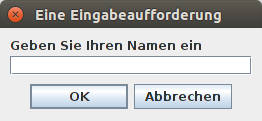
\includegraphics[width=0.3\textwidth]{./media/images/gui/launcher/JOptionPane.png}
  \caption{JOptionPane}
  \label{fig:JOptionPane}
\end{figure}

\begin{lstlisting}[language=JAVA]
String name = JOptionPane.showInputDialog(null,
"Bitte Namen eingeben:",
 " Eingabeaufforderung",JOptionPane.PLAIN_MESSAGE);
p.setName(name);
\end{lstlisting}

Wenn die Eingabe erfolgreich war, wird nun im gewählten Pfad ein neuer Ordner erstellt, welcher das Profil mit dem gewählten Namen repräsentiert. Darin befindet sich eine "`\textit{\textbf{profile.cp}}"' Datei, diese beinhaltet die Benutzereinstellungen. Sobald alle Eingaben getätigt wurden, wird die Entwicklungsumgebung mit dem neu gestalteten Profil gestartet.

Tritt bei der Erstellung eines Profils ein Fehler auf, zeigt eine JOptionpane die zugehörige Fehlermeldung an. Danach öffnet sich automatisch wieder der Lauchner. 

\subsection{Finden eines bereits existierenden Profils}
Damit ein Profil geöffnet werden kann, welches nicht in der Liste der Profile im Launcher vorhanden ist, muss eine Funktion vorhanden sein, mit welcher Profile gefunden werden kann.

Sobald man auf den Button "`\textbf{Finden}"' klickt, wird ein veränderter JFileChooser geöffnet. Hier kann nur eine "`\textit{\textbf{.cp}}"' Datei ausgewählt werden. Sobald diese angeklickt wird, werden das Profilbild und der Profilname als Vorschau auf der rechten Seite angezeigt. Wenn der Nutzer kein Profilbild eingestellt hat, wird hier ein voreingestelltes Profilbild angezeigt.

\begin{figure}[h] 
   \centering
     \includegraphics[width=0.9\textwidth]{./media/images/gui/launcher/launcher_finden.png}
  \caption{ Profilvorschau}
  \label{fig:Bild1}
\end{figure}

Indem man auf den "`\textbf{Öffnen}"'-Button klickt, startet man nun C-Compact mit dem gerade ausgewählten Profil und es wird zu den zuletzt verwendeten Profilen hinzugefügt.


\subsection{Einstellung der Sprache}
\label{sec:win-lang}
Wenn C Compact zum ersten Mal gestartet wird, wird zuallererst dieses Fenster (Abbildung \ref{fig:win-lang}) angezeigt. Der Benutzer wird gebeten, eine Sprache zu wählen. Später kann die Sprache über das Menü \glqq{}Datei\grqq{} im Hauptfenster (Siehe Kapitel \ref{sec:gui-main-menu-file}) geändert werden. Die Änderungen werden erst wirksam, wenn der Benutzer die neue Sprache mit \glqq{}OK\grqq{} bestätigt (siehe auch Kapitel \ref{sec:lang}). Dann wird C Compact neu gestartet.

\begin{figure}[htp]
\centering
\includegraphics[width=0.3\textwidth]{./media/images/gui/elements/Bildschirmfoto-Sprache.png}
\caption{Auswahl der Sprache}
\label{fig:win-lang}
\end{figure}

Dieses Fenster ist in der Klasse \textbf{GUILanguage} im Package \textbf{at.jku.ssw.cmm.gui.properties} implementiert. 

\subsection{Allgemeine Einstellungen}
\label{sec:win-set}
Dieses Fenster (Abbildung \ref{fig:win-set}) enthält allgemeine Optionen zum Haupfenster der Benutzeroberfläche (siehe Kapitel \ref{sec:guimainsettings}). Es kann im Menü des Hauptfensters unter \glqq{}Datei\grqq{} - \glqq{}Einstellungen\grqq{} aufgerufen werden (Siehe Kapitel \ref{sec:gui-main-menu-file}). Änderungen an den Einstellungen werden sofort wirksam (ausgenommen sind Änderungen an der Schriftgröße von Dokumenten). Da C Compact beim Ändern dieser Einstellungen nicht neu gestartet werden muss, sind diese Optionen und die Spracheinstellungen in zwei unterschiedliche Fenster aufgeteilt.

\begin{figure}[htp]
\centering
\includegraphics[width=0.4\textwidth]{./media/images/gui/elements/Bildschirmfoto-Einstellungen.png}
\caption{Einstellungsfenster}
\label{fig:win-set}
\end{figure}

Im Einstellungsfenster können folgende Optionen verändert werden:
\begin{enumerate}
\item \textbf{Ansicht:} Ändert den Aufbau des Hauptfensters. Elemente werden je nach gewähltem Layout unterschiedlich angeordnet. Siehe Kapitel \ref{sec:gui-main-left-ord}.
\item \textbf{Schriftgröße des Sourcecode:} Ändert die Schriftgröße des Textfeldes für den Quellcode im Hauptfenster. Siehe Kapitel \ref{sec:gui-main-left-code}.
\item \textbf{Schriftgröße der Textfelder:} Ändert die Schriftgröße der Textfelder für Ein- und Ausgabedaten im Hauptfenster. Siehe Kapitel \ref{sec:gui-main-left-io}.
\item \textbf{Schriftgröße von Dokumenten:} Dokumente, wie etwa Beschreibungstexte von Fehlern (siehe Kapitel \ref{sec:deb-error}), können mit unterschiedlichen Textgrößen angezeigt werden. Da die Schriftgröße beim Initialisieren der Textfelder festgelegt wird, betrifft die Einstellung immer nur die Dokumente, die in Zukunft geöffnet werden.
\item \textbf{Rückgabewerte anzeigen:} Der Debugger kann den Rückgabewert einer Funktion in einem Popup (siehe auch Kapitel \ref{sec:deb-popup}) darstellen. Da dieses Feature nicht immer hilfreich ist, ist es standardmäßig deaktiviert.
\end{enumerate}

Alle Klassen des Einstellungsfensters befinden sich im Package \textbf{at.jku.ssw.cmm.gui.properties}. Das Fenster selbst wird in der Klasse \textbf{GUIProperties} initialisiert, Listener für alle Schieberregler befinden sich in der Klasse \textbf{PropertiesSliderListener}. Die Combobox für das Layout der Benutzeroberfläche (Option 1) wird mit der Klasse \textbf{PropertiesComboListener} überwacht, die Checkbox für das Anzeigen von Rückgabewerten im Debugger ist mit dem ActionListener \textbf{PropertiesActionListener} verknüpft.

Beim Ändern der Schriftgröße werden zuerst die Einstellungen von C Compact verändert, dann werden die Schriftgrößen in den entsprechenden Elementen aktualisiert.
\begin{lstlisting}[language=JAVA]
@Override
public void stateChanged(ChangeEvent e) {
	JSlider slider = (JSlider)e.getSource();
	
	// Einstellungen aktualisieren
	main.getSettings().setCodeSize(GUIProperties.sliderPosToFont(slider.getValue()));
	
	// Schriftgrößen aktualisieren
	master.updateTextSize();
}
\end{lstlisting}

Tatsächlich wird beim Aktualisieren der Schriftgrößen in Textfeldern einfach ein neuer Font mit der entsprechenden Größe aus dem bereits verwendeten Font abgeleitet und für das Textfeld verwendet.
\begin{lstlisting}[language=JAVA]
// Schriftart (font) ändern
this.jSourcePane.setFont(
	// Aktuellen Font ableiten
	this.jSourcePane.getFont().deriveFont(
		//Schriftgröße laut Einstellungen
		(float)this.main.getSettings().getCodeSize()
	)
);
\end{lstlisting}

\subsection{Über C Compact}
\label{sec:win-credits}
Dieses Fenster (Abbildung \ref{fig:win-about}) enthält den Lizenztext von C Compact sowie die Namen der beteiligten Personen. Auch dieses Fenster kann im Menü der Entwicklungsumgebung aufgerufen werden (Menü siehe Kapitel \ref{sec:gui-main-menu-file}). Alle Bestandteile dieses Elementes befinden sich im Package \textbf{at.jku.ssw.cmm.gui.credits}:
\begin{itemize}
\item \textbf{Credits.java:} Initialisiert das Fenster und regelt sein Verhalten.
\item \textbf{credits.html:} Enthält den Lizenztext.
\item \textbf{credits.css:} Enthält Formatierungsinformationen zum Lizenztext.
\end{itemize}

Die Resourcen sind im Package eingebunden und deshalb auch Teil der generierten JAR-Datei. Dadurch kann der Lizenztext nicht einfach verändert werden.

\begin{figure}[htp]
\centering
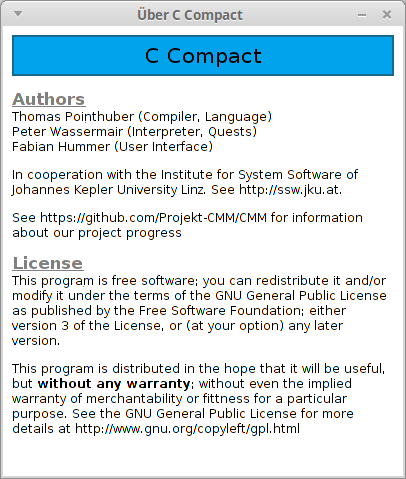
\includegraphics[width=0.4\textwidth]{./media/images/gui/elements/Bildschirmfoto-About.png}
\caption{Fenster mit Lizenztext}
\label{fig:win-about}
\end{figure}

\iffabian
	\subsection{Questpaket auswählen}
	\label{sec:gui-elements-package-sel}
\else
	\section{Questpaket auswählen}
	\label{sec:gui-elements-package-sel}
\fi
%TODO referenz folgt Quest Package erklärung
Hier kann man zwischen den vorhanden Quest Packages (siehe Kapitel \ref{sec:Package}) wählen, wobei rechts die Beschreibung des jeweiligen Packages, falls diese vorhanden ist, angezeigt wird. Mithilfe eines Klicks auf den Pfeil kann das gewünschte Package ausgewählt werden.

\begin{figure}[h] 
  \centering
     \includegraphics[width=1\textwidth]{./media/images/gui/package-auswahl.png}
  \caption{Auswahl des Packages}
  \label{fig:Package_Auswahl}
\end{figure}

Weiters wird auch der Fortschritt des Packages angezeigt. Daraus ist ersichtlich, wie viele Quests man in dem Packet bereits fertiggestellt hat.

Bei einem Quest Package wurde eine JTreeTable (siehe Kapitel: \ref{}) zur Realisierung verwendet. Diese befindet sich wiederum in einer JScrollpane. Somit ist die Anzahl der Elemente in der JTable\footnote{\url{https://docs.oracle.com/javase/tutorial/uiswing/components/scrollpane.html}}  und der JTreeTable nicht begrenzt.


\section{Quest - Selection}
%TODO Referenz Quest System

Sobald ein Package ausgewählt wurde, kann man darin die Quest wählen. Wie beim Questpackage wird rechts die Beschreibung der ausgewählten Quest angezeigt. Der \textbf{"`Type"'} kann in der \textbf{quest.xml} definiert werden. Somit kann man zum Beispiel für verschiedene Aufgabenbereiche verschiedene Attribute verwenden. Links wird der Status der jeweiligen Quest in Symbolen dargestellt.

\begin{figure}[h] 
  \centering
     \includegraphics[width=0.9\textwidth]{./media/images/gui/launcher/package_view.png}
  \caption{Quest Selection}
  \label{fig:Bild1}
\end{figure}

\begin{itemize}
\item Mit einem leeren Feld wird eine nicht gestartete Quest symbolisiert.
\item Eine Uhr bedeutet, dass die Quest bereits gestartet, jedoch noch nicht abgeschlossen wurde.
\item Ein Häkchen symbolisiert eine fertiggestellte Quest.
\item Ein Kreuz bedeutet eine gesperrte Quest. 
\end{itemize}

Die Questzustände werden im Kapitel \ref{sec:Queststate} genauer erklärt.

Sobald eine Quest selektiert wurde, wird der grau hinterlegte \textbf{"`Open"'} Button aktiv und kann nun geklickt werden. Sobald dies geschehen ist, wird die gewählte Quest als aktuelle Quest ins Profil übernommen und C Compact dementsprechend angepasst. Die Quest wird somit gestartet.

Zur Realisierung wurde eine JTable verwendet. Diese befindet sich wiederum in einer JScrollpane. Das Questpackage und die Questselection verwenden grundsätzlich dasselbe JFrame. Beim Wechseln auf die JTable, muss die JTreeTable entfernt werden. Danach kann der neue JTable hinzugefügt werden.
\begin{lstlisting}[language=JAVA]
	public void changetoQuestTable(){
		splitpane.remove(jTablePanel);
		splitpane.setLeftComponent(inittable());

		frame.validate();
		frame.repaint();
	}
\end{lstlisting}

%Mithilfe der \textit{frame.validate()} Methode wird noch einmal überprüft, ob alle Komponenten ordnungsgemäß zugewiesen werden. Danach muss das gesamte JFrame neu gezeichnet werden, was in diesem Fall von der \textit{frame.repaint()}-Methode durchgeführt wird.

\subsection{Dialoge}
\label{sec:win-dialog}
In C Compact werden viele verschiedene Dialogfenster verwendet. Der Begriff Dialogfenster\footnote{http://de.wikipedia.org/wiki/Dialog\_(Benutzeroberfläche)} umfasst eine Reihe von unterschiedlichen Anwendungen, bei denen ein Fenster verwendet wird, um Informationen oder Befehle vom Benutzer einzuholen. Dialoge werden in C Compact beispielsweise verwendet, um zu fragen, ob eine Datei gespeichert werden soll (Abbildung \ref{fig:win-dialog}), oder um den Benutzer auf ein Problem aufmerksam zu machen. Swing enthält bereits einige Funktionen zum Erstellen von Dialogen\footnote{http://docs.oracle.com/javase/tutorial/uiswing/components/dialog.html}, anhand der offiziellen Tutorials können einfache Dialoge sehr schnell erstellt werden.

\begin{figure}[htp]
\centering
\includegraphics[width=0.4\textwidth]{./media/images/gui/elements/Bildschirmfoto-Dialog.png}
\caption{Ein einfacher Dialog}
\label{fig:win-dialog}
\end{figure}

\subsection{Dateimanager}
\section{JFileChooser}
\label{sec:JFileChooser}

Der JFileChoosers\footnote{\url{http://docs.oracle.com/javase/7/docs/api/javax/swing/JFileChooser.html}} ermöglicht dem Benutzer, Dateien und Ordner auszuwählen. Dieser kann mit den verschiedensten Methoden angepasst werden.
\begin{lstlisting}[language=JAVA]
JFileChooser chooser = new JFileChooser();
\end{lstlisting}
    
Nun kann man verschiedenste Einstellungen vornehmen. Sehr oft wurde von uns ein sogenannter FileNameExtensionFilter verwendet. Mit diesem ist es möglich, Dateien mit bestimmten Endungen herauszufiltern und nur diese anzeigen zu lassen.

Dies wurde zum Beispiel beim Suchen nach C-Compact Profilen verwendet!
\begin{lstlisting}[language=JAVA]
FileFilter filter = new FileNameExtensionFilter("CMM Profile",".cp");
chooser.setFileFilter(filter);
\end{lstlisting}



\subsection{Anzeigen einer Vorschau}
Bei der Verwendung des JFileChoosers wurde oftmals ein Zusatz hinzugefügt, der es dem Nutzer ermöglicht, eine Vorschau\footnote{\url{http://www.javalobby.org/java/forums/t49462.html}} eines Bildes sowie den Nutzernamen zu sehen.

Die Vorschau wird in einer Klasse erstellt, welche ein JPanel erweitert und den PropertyChangeListener implementiert. Beim Anlegen des Konstruktors ist darauf zu achten, dass das JPanel bereits im Konstruktor eine geeignete Größe zugewiesen bekommt.

%TODO FIX
Zuerst wird die Methode PropertyChange aufgerufen, welches beim Klicken auf eine Datei oder einen Ordner erscheint. Nun wird die Variable, welche der Methode übergeben wurde, auf ein File umgeändert. Somit kann nun abgefragt werden, ob es sich hierbei um den gewünschten Datentyp handelt. Danach wird die \textit{repaint()} Methode benötigt, um die \textit{paintComponent()} Methode aufzurufen.
\begin{lstlisting}[language=JAVA]
	public void propertyChange(PropertyChangeEvent e) {
		String propertyName = e.getPropertyName();

		if (propertyName.equals(JFileChooser.SELECTED_FILE_CHANGED_PROPERTY)) {
			File selection = (File) e.getNewValue();
			...
			}
\end{lstlisting}

% http://www.javalobby.org/java/forums/t49462.html
In weiterer Folge muss das Bild nur mehr geladen und skaliert werden. Mithilfe der paintComponent Methode kann das Bild nun eingeschleust werden. Hierfür wird die \textit{drawImage} Methode verwendet. Dabei ist zu beachten, dass das Bild im JPanel in der richtigen Position gezeichnet wird.
\begin{lstlisting}[language=JAVA]
public void paintComponent(Graphics g) {
		g.setColor(bg);
		g.fillRect(0, 0, ACCSIZE, getHeight());
		g.drawImage(image, getWidth() / 2 - width / 2 + 5, getHeight() / 2
				- height / 2, this);
		
	}
\end{lstlisting}

Nun kann die neue Klasse eingebunden werden. Dies geschieht, indem man mehrere vorgegebene Klassen verwendet. Hierbei steht \textit{setAccessory()} für extra Komponenten, und \textit{PropertyChangeListener()} ist für Events, die im JFileChooser ausgeführt werden, zuständig.

\begin{lstlisting}[language=JAVA]
		ProfilePreviewPanel preview = new ProfilePreviewPanel();
		chooser.setAccessory(preview);
		chooser.addPropertyChangeListener(preview);
\end{lstlisting}

Wenn alle Veränderungen vorgenommen wurden, kann der FileChooser mit \textit{showdialog()}- angezeigt und die gewünschten Daten abgefragt werden.

\section{Einstellungen}
\label{sec:guimainsettings}
Für den Betrieb einer Benutzeroberfläche ist es unerlässlich, diese anpassbar zu machen und Änderungen des Benutzers zu speichern. Im Package \textbf{at.jku.ssw.cmm.gui.properites} befindet sich die Klasse \textbf{GUImainSettings}, die alle globalen Einstellungen verwaltet und speichert. Diese Einstellungen umfassen:
\begin{itemize}
\item Die zuletzt geöffneten Dateien
\item Die gerade geöffnete Datei
\item Die zuletzt geöffneten Benutzerprofile
\item Das gerade aktive Benutzerprofil
\item Die vom Benutzer gewählte Sprache (siehe Kapitel \ref{sec:lang})
\item Einstellungen, die der Benutzer direkt verändern kann (Siehe Kapitel \ref{sec:win-set})
\begin{itemize}
\item Schriftgrößen
\item Layout der Benutzeroberfläche
\end{itemize}
\end{itemize}

Bevor das Hauptfenster der Entwicklungsumgebung gestartet werden kann, muss ein Objekt der Klasse \textbf{GUImainSettings} erstellt werden (Siehe dazu Kapitel \ref{sec:gui-main-impl}). Dabei werden die zuletzt gespeicherten Konfigurationen geladen.

Die Einstellungen werden in der Datei \textbf{settings.xml} im Hauptverzeichnis von C Compact gespeichert. Bevor diese Datei ausgelesen wird, werden alle Einstellungsvariablen auf einen definierten Standardwert gesetzt. Sollten bestimmte Informationen oder die Datei selbst fehlen, werden die Standardwerte wieder hergestellt. Die Einstellungen werden beim Beenden von C Comapct gespeichert.

Das Lesen von XML-Dateien wird in Kapitel \ref{sec:xml-read} beschrieben, das Schreiben in Kapitel \ref{sec:xml-write}. 

Die Einstellungsdatei \textbf{settings.xml} ist wie folgt aufgebaut:
\begin{lstlisting}[language=XML]
<?xml version="1.0" encoding="UTF-8" standalone="no"?>
<settings xmlns="settings.xml">
	<properties>
		<language>de</language>
		<codesize>16</codesize>
		<textsize>16</textsize>
		<varsize>16</varsize>
		<varoffset>0</varoffset>
		<descsize>0</descsize>
		<returnpopup>false</returnpopup>
	</properties>
	<lastfile>/home/fabian/Dokumente/C--/C_Compact_Alpha_1.4.5/examples/helloworld/helloworld.cmm</lastfile>
	<lastfile>/home/fabian/Dokumente/C--/C_Compact_Alpha_1.4.5/examples/random/random.cmm</lastfile>
	<lastfile>/home/fabian/Dokumente/C--/C_Compact_Alpha_1.4.5/examples/bubblesort/bubblesort.cmm</lastfile>
	<profile>/home/fabian/Dokumente/profile_Fabian</profile>
</settings>
\end{lstlisting}

Unter \glqq{}properties\grqq{} befinden sich alle Parameter, die der Benutzer direkt ändern kann (die Sprache bei den Spracheinstellungen, siehe Kapitel \ref{sec:win-lang} und alle anderen Einstellungen bei den allgemeinen Einstellungen, siehe Kapitel \ref{sec:win-set}). Darunter werden die zuletzt gewählten Profile aufgelistet (diese werden im Launcher angezeigt, siehe Kapitel \ref{sec:win-launcher}) und dann die zuletzt geöffneten Dateien (für die Auflistung im Menü der Entwicklungsumgebung, siehe Kapitel \ref{sec:gui-main-menu-ctrl}). Damit die Listen nicht zu lang werden, werden nur die letzten 10 geöffneten Dateien und die letzten 10 aktiven Profile gespeichert und angezeigt.

\section{Übersetzungen}
\label{sec:lang}
C Compact ist derzeit in zwei Sprachen erhältlich: Englisch und Deutsch. Die Texte in der jeweiligen Sprache werden beim Initialisieren der Benutzeroberfläche geladen. Deshalb muss C Compact neu gestartet werden, wenn eine andere Sprache ausgewählt wird (siehe Kapitel \ref{sec:win-lang}).

Zum Erstellen der Übersetzungsdateien wurde GNU gettext\footnote{http://www.gnu.org/software/gettext/} verwendet. Auf Debian-basierten Linux-Systemen (wie zum Beispiel Ubuntu oder Linux Mint) kann gettext einfach über die Paketverwaltung installiert werden:
\begin{lstlisting}[language=sh]
apt-get install gettext
\end{lstlisting}

Dieses Projekt beinhaltet Programme zum Extrahieren von zu übersetzenden Strings aus Quelldateien. Mit dem Befehl \textbf{xgettext}\footnote{http://www.gnu.org/savannah-checkouts/gnu/gettext/manual/html\_node/xgettext-Invocation.html} werden alle zu übersetzenden Strings aus den Quelldateien ausgelesen und in eine externe Datei gespeichert.
\begin{lstlisting}[language=sh]
xgettext -k_ -o po/keys.pot $(find src -name "*.java")
\end{lstlisting}
Dieser Befehl muss aus dem Projektordner ausgeführt werden. Dabei wird im Quelltext des Projektes nach Schlüsselwörtern gesucht, die auf einen zu übersetzenden Text hindeuten. Mit dem Parameter \emph{-k[keyword]} wird das Schlüsselwort angegeben, in diesem Fall \glqq{}\_\grqq{}. Mit dem Parameter \emph{-o file} wird die Ausgabedatei angegeben. Die zu übersetzenden Strings werden hier in die Datei po/keys.pot gespeichert.

Der Befehl \textbf{msgmerge} fügt die Texte aus dieser Datei in eine Datei für Übersetzungen ein. Befinden sich in dieser Datei bereits übersetzte Texte, werden die neuen Strings einfach hinzugefügt.
\begin{lstlisting}[language=sh]
msgmerge -U po/de.po po/keys.pot
\end{lstlisting}

In der erstellten Datei --- in diesem Fall \textbf{de.po} im Ordner \textbf{po} --- werden die Texte nacheinander aufgelistet. Neben dem Schlüsselword \textbf{msgid} steht immer der Originaltext, der übersetzte Text ist in \textbf{msgstr} einzutragen. Über jeder Übersetzung stehen außerdem Kommentare mit den Ursprungsdateien dieses Textes.
\begin{lstlisting}[language=sh]
#: src/at/jku/ssw/cmm/launcher/GUILauncherMain.java:135
#: src/at/jku/ssw/cmm/gui/properties/GUILanguage.java:40
msgid "Welcome"
msgstr "Willkommen"
\end{lstlisting}

Damit das Einfügen von neuen Strings mit dem Befehl \textbf{msgmerge} auch mit Umlauten funktioniert, müssen bei den allgemeinen Informationen zu Beginn der Übersetzungsdatei Codierungsvorschriften eingefügt werden.
\begin{lstlisting}[language=sh]
"Content-Type: text/plain; charset=ISO-8859-15\n"
"Content-Transfer-Encoding: 8bit\n"
\end{lstlisting}

Die Übersetzungsfunktionen sind in der Klasse \textbf{at.jku.ssw.cmm.gettext.Language} impementiert. Vor dem Initialisieren muss die Methode \textbf{loadLanguage} aufgerufen werden. Als Parameter wird der Name der Datei mit den Übersetzungen übergeben, zum Beispiel \glqq{}de.po\grqq{}.
\begin{lstlisting}[language=JAVA]
Language.loadLanguage("de.po");
\end{lstlisting}

Alle Übersetzungen werden in eine HashMap gespeichert. Der Schlüssel ist der Text in Originalsprache (Englisch), zugehöriger Datenwert ist der übersetzte String. Mit der Methode \glqq{}\_(...)\grqq{} können Übersetzungen abgefragt werden. Wurde keine Sprache geladen, wird der Originalstring zurückgegeben. Ist keine Übersetzung für einen bestimmten Text vorhanden, wird ebenfalls der Schlüsseltext zurückgegeben, allerdings wird auch eine Warnung in der Konsole ausgegeben. Nicht übersetzte Strings werden also einfach in Originalsprache angezeigt.
\begin{lstlisting}[language=JAVA]
jLabel.setText(_("Wilkommen"));
\end{lstlisting}

Um die Übersetzungsmethode verwenden zu können, ohne davor den Klassennamen zu schreiben, muss die Methode statisch importiert werden:
\begin{lstlisting}[language=JAVA]
import static at.jku.ssw.cmm.gettext.Language._;
\end{lstlisting}

\section{Anzeigen von internen Fehlern}
\label{sec:gui-int-error}
Unter Umständen kann es bei C Compact zu internen Fehlern kommen. Zu diesen zählen Probleme die entstehen, wenn eine wichtige Datei nicht gefunden werden kann. Die in diesem Abschnitt beschriebenen Fehlermeldungen sollten nicht mit den Fehlerbeschreibungen des Debuggers verwechselt werden (Siehe Kapitel \ref{sec:deb-error}). Wenn ein Fehler auftritt, wird die Fehlermeldung in Form eines Dialoges (Siehe Kapitel \ref{sec:win-dialog}) angezeigt.

\begin{figure}[htp]
\centering
\includegraphics[width=0.5\textwidth]{./media/images/gui/elements/Bildschirmfoto-Error-Message.png}
\caption{Eine interne Fehlereldung}
\end{figure}

Jeder Fehler der auftreten kann hat eine eindeutige Fehlernummer. Alle Fehler sind in der C Compact Projektwiki auf GitHub\footnote{https://github.com/Projekt-CMM/CMM/wiki/List-of-internal-error-numbers} aufgelistet. Eine Fehlernummer besteht immer aus 4 Zahlen; die erste gibt den Bereich von C Compact an, in dem der Fehler aufgetreten ist.

Die Anzeigetexte und Fehlernummern werden in der Datei \textbf{systemerror.xml} gespeichert. Diese Datei befindet sich im Package \textbf{at.jku.ssw.cmm.gui.debug} und wird damit auch in die fertige JAR-Datei eingebunden. So kann sie nicht aus Versehen gelöscht werden.

Um eine Fehlermeldung anzeigen zu können muss einfach folgender Befehl ausgeführt werden:
\begin{lstlisting}[language=JAVA]
// Parameter: JFrame des Hauptfensters, Fehlernummer, Sprachcode (zum Beispiel "de" oder "en")
new ErrorMessage().showErrorMessage(jFrame, "#2001", settings.getLanguage());
\end{lstlisting}

\def\arraystretch{1.6}
\begin{minipage}{14cm}
%\begin{table}[ht]
\begin{tabular}{l|l|l}
	Bereich&Nummer&Beschreibung\\
	\hline
	&1001&Datei \textbf{error/table.xml} fehlt\\
	\multirow{5}{15mm}{\begin{sideways}\parbox{35mm}{Dateien fehlen oder sind beschädigt}\end{sideways}}&1002&Inhalt der Datei \textbf{error/table.xml} ist ungültig (ParserException)\\
	&1003&Inhalt der Datei \textbf{error/table.xml} ist ungültig (SAXException)\\
	&1011&Datei \textbf{error/style.css} fehlt oder ist beschädigt\\
	&1012&Inhalt der Datei \textbf{error/style.css} ist ungültig\\
	&1021&Fehlerbeschreibungsdokument nicht gefunden\\
	\hline
	&2001&Aktuelle Datei konnte nicht gespeichert werden\\
	\multirow{4}{15mm}{\begin{sideways}\parbox{25mm}{Dateien öffnen oder speichern}\end{sideways}}&2011&[inactive]\footnote{Dieser Fehler kann nicht mehr auftreten, da der zugehörige Bereich deaktiviert wurde}\\
	&2012&Datei konnte nicht geöffnet werden\\
	&2013&Bibliothek konnte nicht gefunden werden\footnote{Dieser Fehler wird als Fehlermeldung im Debugger angezeigt. Die Fehlernummer existiert nur formell}\\
	&2014&Datei \textbf{default.cmm} einer Quest konnte nicht geöffnet werden\\
	\hline
	&3001&Exception im Präprozessor\\
	\multirow{4}{15mm}{\begin{sideways}\parbox{25mm}{Testen einer Quest}\end{sideways}}&3002&[inactive]\footnote{Dieser Fehler kann nicht mehr auftreten} IOException im Präprozessor\\
	&3003&Unbekannter Fehler im Präprozessor\\
	&3004&Compiler wurde unerwartet beendet (Exception)\\
	&3005&Compiler durch Fehler im Sourcecode abgebrochen\\
	\hline
	\parbox{23mm}{Verbindungs- probleme}&9001&Fehler beim Drucken
\end{tabular}
%\caption{Interne Fehlernummern}
%\label{tab:int-err}
%\end{table}
\end{minipage}